\chapter{Resuelves problemas de semejanza de triángulos y teorema de pitágoras}

\section{Triángulos semejantes}

\subsection{Definición}

Dos triángulos $ABC$ y $DEF$ son semejantes si tiene una de las propiedades
equivalentes:

\begin{itemize}
\item $\widehat{A} = \widehat{D}, \widehat{B} = \widehat{E},
  \widehat{C} = \widehat{F}$
\item $\frac{DE}{AB} = \frac{EF}{BC} = \frac{FD}{CA}$
\end{itemize}

\subsection{Ejercicio 1}

Encontre dos triángulos semejantes que no son congruentes.
¿Es la recíproca posible?

\subsection{Ejercicio 2}

Sean dos triángulos $ABC$ y $DEF$.

\begin{enumerate}
\item Mostrar que
  si $\widehat{A} = \widehat{D}, \widehat{B} = \widehat{E}$, son semejantes.
\item ¿Que decir si sólo tenemos $\widehat{A} = \widehat{D}$?
\item ¿Y si sólo tenemos $\frac{DE}{AB} = \frac{EF}{BC}$?
\end{enumerate}

\subsection{Teorema de Tales}

Si en un triángulo se traza una línea paralela a cualquiera de sus lados, se
obtiene un triángulo que es semejante al triángulo dado.

Por ejemplo, en la figura siguiente, consideramos un triángulo $ABC$ y trazamos
3 rectas (roja, verde y azul) paralela al lado $AB$. Obtenemos tres
triángulos ${A_1B_1C_1}, {A_2B_2C_2}, {A_3B_3C_3}$ semejantes a $ABC$:

\begin{center}
 \begin{tikzpicture}
   \draw (0,0)node[below left] {$A$} -- (0,4) node[above left] {$B$}
   -- (3,1) node[right] {$C$} -- (0,0)[color=orange];
   \draw (6,-2) -- (3,1) -- (6,2)[dashed];
   \draw (0,0) -- (-3,-1)[dashed];
   \draw (0,4) -- (-3,7)[dashed];

   \draw (-1,7) -- (-1,5)node[above left] {$B_1$} --
   (-1,-0.33333333333333)node[below left] {$A_1$} -- (-1,-3)[red];
   \draw (2,7) -- (2,2)node[above right] {$B_2$} --
   (2,0.66666666666666)node[below right] {$A_2$} -- (2,-3)[green];
   \draw (5,7) -- (5,1.66666666666666)node[above right] {$A_3$}
   -- (5,-1)node[below right] {$B_3$} -- (5,-3)[blue];
   \
 \end{tikzpicture}
\end{center}

y tenemos:

$$
\frac{CA}{CA_1} = \frac{CB}{CB_1} = \frac{AB}{A_1B_1}
$$
%%
$$
\frac{CA_2}{CA} = \frac{CB_2}{CB} = \frac{A_2B_2}{AB}
$$
%%
$$
\frac{CA}{CA_3} = \frac{CB}{CB_3} = \frac{AB}{A_3B_3}
$$

\subsection{Ejercicio 3 (Tales)}

En la figura precedente, utilice los resúltados del cápitulo uno para explicar
por que

\begin{enumerate}
\item ¿$\widehat{BCA} = \widehat{B_3CA_3}$?
\item ¿$\widehat{CA_3B_3} = \widehat{CAB}$ y $\widehat{CB_3A_3} = \widehat{CBA}$?
\item ¿$\widehat{CA_1B_1} = \widehat{CA_2B_2} = \widehat{CAB}$ y
  $\widehat{CB_1A_1} = \widehat{CB_2A_2} = \widehat{CBA}$?
\end{enumerate}

Deducir el teorema de Tales.

\subsection{Ejercicio 4 (pirámide de Keops)}

Según la leyenda, Tales de Mileto empleó su teorema para medir la altura de la
pirámide de Keops:

\begin{center}
\includegraphics{cheops.png}\\
Fuente: Wikimedia Commons
\end{center}

Determine la altura de la pirámide a partir de esas medidas:

\begin{itemize}
  \item altura de la vara: 1.63m.
  \item sombra de la vara: 2m.
  \item longitud de la base de la pirámide: 230m.
  \item sombra de la pirámide: 65m.
\end{itemize}

\subsection{Ejercicio 5 (números constructibles)}

En este ejercicio, consideramos un segmento unidad sobre una hoja de papel y
queremos construir otra longitudes, utilizando sólo regla y compás.

\begin{center}
 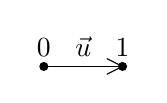
\begin{tikzpicture}
   \draw (0,0)node[above]{$0$} -- (0.5,0)node[above]{$\vec{u}$} -- (1,0)node[above]{$1$};
   \draw (.8,.1) -- (1,0) -- (.8,-.1);
   \draw[fill=black] (0,0) circle(.05);
   \draw[fill=black] (1,0) circle(.05);
 \end{tikzpicture}
\end{center}

Indique cómo construir los ńumeros naturales $0, 1, 2, 3, 4, 5, \ldots$.

\begin{center}
 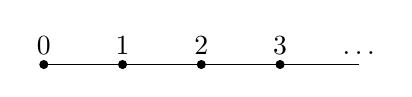
\begin{tikzpicture}
   \draw (0,0)node[above]{$0$} -- (1,0)node[above]{$1$}
   -- (2,0)node[above]{$2$} -- (3,0)node[above]{$3$}
   -- (4,0)node[above]{$\ldots$};
   \draw[fill=black] (0,0) circle(.05);
   \draw[fill=black] (1,0) circle(.05);
   \draw[fill=black] (2,0) circle(.05);
   \draw[fill=black] (3,0) circle(.05);
 \end{tikzpicture}
\end{center}

Indique cómo construir el eje ortogonal, de los números imaginarios puros:

\begin{center}
 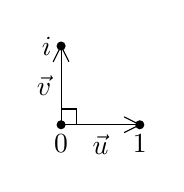
\begin{tikzpicture}
   \draw (0,0)node[below]{$0$} -- (0.5,0)node[below]{$\vec{u}$} -- (1,0)node[below]{$1$};
   \draw (.8,.1) -- (1,0) -- (.8,-.1);
   \draw (0,0) -- (0,0.5)node[left]{$\vec{v}$} -- (0,1)node[left]{$i$};
   \draw (.1,.8) -- (0,1) -- (-.1,.8);
   \draw[fill=black] (0,0) circle(.05);
   \draw[fill=black] (1,0) circle(.05);
   \draw[fill=black] (0,1) circle(.05);
   \draw (0,.2) -- (.2,.2) -- (.2,0);
 \end{tikzpicture}
\end{center}

Ahora, consideramos dos enteros distinctos $p, q > 0$. Sea $D$ la recta (roja)
pasando por los puntos $(q,0)$ y $(0,1)$.
Indicar cómo trazar la recta (ázul) pasando por $(p,0)$ recta, paralela a $D$.

\begin{center}
 \begin{tikzpicture}
   \draw (0,0)node[below]{$0$} -- (0.5,0)node[below]{$\vec{u}$} -- (1,0)node[below]{$1$} -- (8,0);
   \draw (.8,.1) -- (1,0) -- (.8,-.1);
   \draw (0,0) -- (0,0.5)node[left]{$\vec{v}$} -- (0,1)node[left]{$i$} -- (0,5);
   \draw (.1,.8) -- (0,1) -- (-.1,.8);
   \draw[fill=black] (0,0) circle(.05);
   \draw[fill=black] (1,0) circle(.05);
   \draw[fill=black] (0,1) circle(.05);
   \draw (0,.2) -- (.2,.2) -- (.2,0);


   \draw[fill=black] (3,0) circle(.05) node[below]{$q$};
   \draw[fill=black] (7,0) circle(.05) node[below]{$p$};


   \draw[color=red] (-3,2) -- (6,-1);
   \draw[color=blue] (-3,3.333333333333333) -- (7,0);

 \end{tikzpicture}
\end{center}

¿Cual es el punto de intersección de esta recta ázul con el eje de 
de los números imaginarios puros? Deducir que todos los números racionales
son constructibles con regla y compás.

\section{Teorema de Pitágoras}

\subsection{Definición}

En un triángulo rectángulo, los catetos son los lados menores y la hipotenusa
es lado mayor.

\subsection{Teorema}

En todo triángulo rectángulo el cuadrado de la hipotenusa es igual a la suma de
los cuadrados de los catetos. 

\begin{center}
 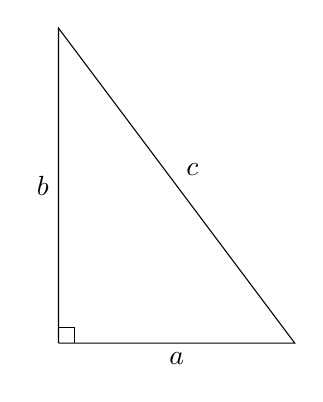
\begin{tikzpicture}
   \draw (0,0) --
   (1.5,0)node[below]{$a$} -- (3,0) --
   (1.5,2)node[above right]{$c$} -- (0,4) --
   (0,2)node[left]{$b$} -- (0,0);
   \draw (0,.2) -- (.2,.2) -- (.2,0);
 \end{tikzpicture}
\end{center}

$$
a^2 + b^2 = c^2
$$

\subsection{Ejercicio 6}

Determine las longitudes $a,b,c$ de los lados de un triángulo rectángulo
(figura arriba), si

\begin{enumerate}
\item ¿$a = 12, b = 35$?
\item ¿$b = 56, c = 65$?
\item ¿$a = 11, c = 61$?
\end{enumerate}

\subsection{Ejercicio 7}

Consideramos la figura siguiente:

\begin{center}
 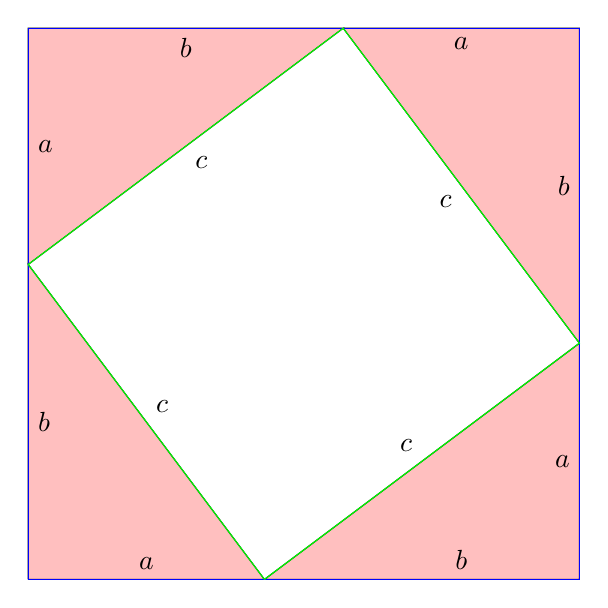
\begin{tikzpicture}

   \draw[color=black,fill=pink]
   (0,0) --
   (1.5,0)node[above]{$a$} -- (3,0) --
   (1.5,2)node[above right]{$c$} -- (0,4) --
   (0,2)node[right]{$b$} -- (0,0);

   \draw[color=black,fill=pink]
   (0,4) --
   (0,5.5)node[right]{$a$} -- (0,7) --
   (2,7)node[below]{$b$} -- (4,7) --
   (2,5.5)node[below right]{$c$} -- (0,4);

   \draw[color=black,fill=pink]
   (4,7) --
   (5.5,7)node[below]{$a$} -- (7,7) --
   (7,5)node[left]{$b$} -- (7,3) --
   (5.5,5)node[below left]{$c$} -- (4,7);

   \draw[color=black,fill=pink]
   (7,3) --
   (7,1.5)node[left]{$a$} -- (7,0) --
   (5.5,0)node[above]{$b$} -- (3,0) --
   (5,1.5)node[above left]{$c$} -- (7,3);

   \draw[color=blue]
   (0,0) -- (7,0) -- (7,7) -- (0,7) -- (0,0);

   \draw[color=green]
   (3,0) -- (7,3) -- (4,7) -- (0,4) -- (3,0);

 \end{tikzpicture}
\end{center}

Expresar en función de $a,b,c$:

\begin{itemize}
  \item La area $A$ del pequeño cuadrado (verde).
  \item La area $C$ del grán cuadrado (azul).
  \item La area rosa $B$ (cuatro triángulos rectángulos).
\end{itemize}

De la igualidad $C = A + B$ deduce el teorema de Pitágoras $c^2 = a^2 + b^2$.

\subsection{Ejercicio 8 (contruir una raíz cuadrada)}

Suponemos que tenemos una longitud unidad y otra longitud $x$.
Explique cómo obtener la figura siguiente con regla y compás:

\begin{center}
 \begin{tikzpicture}
   \draw[color=red, dashed] (10,0) arc (0:180:5);
   \draw(1.2,0) -- (1.2,.2) -- (1,.2);

   \draw(0,0) -- (0.5,0)node[below]{$1$} -- (1,0) --
   (5.5,0)node[below]{$x$} -- (10,0);
   \draw(1,0) -- (1,1.5)node[right]{$h$} -- (1,3);
   \draw(1,3) -- (5.5,1.5)node[above right]{$b$} -- (10,0);
   \draw(1,3) -- (.5,1.5)node[above left]{$a$} -- (0,0);

   \draw[color=blue]
   (0,-.5) -- (0,-1) -- (5,-1)node[below]{$c = 1 + x$} -- (10,-1) -- (10, -.5);
 \end{tikzpicture}
\end{center}

Un teorema de Tales dice que el triángulo inscrito en el círculo rojo,
de lados $a, b, c$ es rectángulo (ejercicio 6 del primer cápitulo).
Utilice el Teorema de Pitágoras sobre este
triángulo y dos otros para obtener la relación $h = \sqrt{x}$.

\subsection{Ejercicio 9}

Utilice las técnicas de los ejercicios 5 y 8 para construir
$x = \frac{17}{3}$, $p = \sqrt{17}$, $q = \sqrt{3}$, $\sqrt{x}$ y $\frac{p}{q}$.
Verifique geometricamente que 
%%
$$
\sqrt{\frac{17}{3}} = \frac{\sqrt{17}}{\sqrt{3}}
$$

\section{Soluciones de los ejercicios}

\subsection{Ejercicio 1}

Por ejemplo, dos triángulos $ABC$ y $AEF$ rectángulos en $A$ con
$1 = {AB} = {AC} = \frac{AE}{2} = \frac{AF}{2}$ tienen ángulos
$(90°, 45°, 45°)$ pero sus lados no son de misma longitud.

La recíproca es imposible: si $ABC$ y $DEF$ son congruentes, tenemos
$\frac{DE}{AB} = \frac{EF}{BC} = \frac{FD}{CA} = 1$.

\subsection{Ejercicio 2}

\begin{enumerate}
\item Tenemos
  $\widehat{C} = {180° - \widehat{A} - \widehat{B}} =
  {180° - \widehat{D} - \widehat{E}} = \widehat{F}$ y entonces
  los triángulos son semejantes.
\item Es fácil encontrar dos triángulos con $\widehat{A} = \widehat{D}$
  pero los otros ángulos que no coresponden.
\item Considerar por ejemplo $A = D$, $B = E$ y $AB = AC = DF$ pero
  $90° = \widehat{A} \neq \widehat{D} = 135°$.
\end{enumerate}

\subsection{Ejercicio 3 (Tales)}

\begin{enumerate}
\item Son ángulos opuestos por el vertice.
\item Son ángulos alternos.
\item Son ángulos corespondientes.
\end{enumerate}

De estas igualides de ángulos, vemos que $A_1B_1C_1$, $A_2B_2C_2$ y
$A_3B_3C_3$ son semejantes a $ABC$.

\subsection{Ejercicio 4 (pirámide de Keops)}

Los radios del sol son paralelas y por lo tanto podemos mover la vara para
que las extremidades de las sombras coincida al mismo punto. Podemos aplicar
el teorema de Tales:

$$
\frac{B}{C} = \frac{A}{D}
$$
%%
entonces $D = \frac{A C}{B} = \frac{1.63 \times
  \left(\frac{230}{2}+65\right)}{2} = 146.7m$

\subsection{Ejercicio 5 (números constructibles)}

Trazamos con la regla el eje pasando por los puntos $(0,0)$ y $(1,0)$. Con el
compás, podemos reportar la longitud del segmento inicial sobre este eje para
obtener los puntos $(2,0)$, $(3,0)$ etc que coresponden a los números naturales.

El eje ortogonal, de los ńumeros imaginarios puros es la mediatriz del segmento
$[-1,1]$. El punto $-1$ se contruye de la misma manera que los números
naturales. Con el compás, trazamos los círculos de centros $-1$ y $1$ y de
radio $2$. Se cortan en dos puntos sobre la mediatriz que podemos trazar con
la regla.

Con el compás, reportamos longitud del segmento inicial
sobre el eje de los ńumeros imaginarios puros para obtener el punto $(0,1)$ que
coresponde al ńumero complejo $i$. Con la regla, trazamos la recta roja pasando
por $(q,0)$ y $(0,1)$.

El círculo de centro $(p,0)$ y de radio $r=|p-q|$ corta la recta $D$ en
$Q_1={(q,0)}$ y otro punto $Q_2$. Con la técnica arriba, podemos trazar la
mediatriz de $[Q_1Q_2]$, que es la recta $D'$
ortogonal a $D$ pasando por ${(p,0)}$. El círculo de radio $1$ y centro
$(p,0)$ corta esta recta $D'$ en dos puntos $P_1, P_2$. De nuevo, trazamos
la mediatriz de $[P_1P_2]$: es la recta pasando por $(p,0)$ y paralela a
$D$, es decir la recta ázul.

La recta ázul intesecta el eje de los imaginarios puros en un punto
$(0,x)$ donde $x > 0$. Por el teorema de Tales, obtenemos
%%
$$
x = \frac{x}{1} = \frac{p}{q}
$$

Con el compás, podemos reportar esta longitud $x$ sobre el eje original para
obtener el punto $\left(\frac{p}{q}, 0 \right)$ corespondiente al racional
$\frac{p}{q}$. De la misma manera, obtenemos $-\frac{p}{q}$
Los casos $p = 0$ y $p = q$ coresponden a los puntos originales $0, 1$.
Entonces, podemos contruir todos los números racionales.

\subsection{Ejercicio 6}

\begin{enumerate}
\item $c = \sqrt{12^2 + 35^2} = 37$
\item $a = \sqrt{65^2 - 56^2} = 33$
\item $b = \sqrt{61^2 - 11^2} = 60$
\end{enumerate}

\subsection{Ejercicio 7}

\begin{itemize}
  \item $A = c^2$
  \item $C = \left(a+b\right)^2 = a^2 + {2ab} + b^2$
  \item $B = 4 \times \frac{ab}{2} = {2ab}$
\end{itemize}

Entonces $a^2 + b^2 = C - B = A = c^2$.

\subsection{Ejercicio 8 (contruir una raíz cuadrada)}

Trazamos una recta donde reportamos las longitudes $1$ y $x$ para obtener
un segmento de longitud $c = 1 + x$. Trazamos la mediatriz (ver ejercicio 5)
de este segmento para obtener el centro de círculo rojo que podemos dibujar con
el compás. Reportamos la unidad de referencia sobre el segmento para obtener
los puntos de coordenadas $0$ y $2$. La mediatriz del segmento formado por estos
puntos intersecta el círculo rojo para dar la nueva longitud $h$.

Las relaciones de Pitágoras se escriben:

$$c^2 = a^2 + b^2$$
$$a^2 = 1^2 + h^2$$
$$b^2 = x^2 + h^2$$

Entonces
${1^2+h^2 + x^2 + h^2} = a^2 + b^2 = c^2 = {(1+x)}^2 = 1^2+2x+x^2$,
$2h^2 = 2x$ y finalmente, $h = \sqrt{x}$.

\subsection{Ejercicio 9}

$x = \frac{17}{3}$ se obtene por la técnica del ejercicio 5.
$p = \sqrt{17}$, $q=\sqrt{3}$ y $\sqrt{x}$ se obtenen por la técnica del
ejercicio 8. Finalmente, $\frac{p}{q}$ se obtene como en el ejercicio 5
(no necesitamos que $p,q$ sean enteros para hacer la construción). Podemos
verificar que las longitudes $\sqrt{x}$ y $\frac{p}{q}$ son iguales.

